% !TEX program = xelatex

\documentclass[12pt]{article} % 基础字号设定为12pt
\usepackage[margin=2.25cm]{geometry} % 页面边距

% 字体与中文支持
\usepackage{xeCJK}
\setmainfont{Garamond}
\setCJKmainfont{SimSun} % 中文默认字体 宋体
\setCJKsansfont{SimHei} % 中文无衬线字体 黑体

% 常用宏包
\usepackage{graphicx}
\usepackage{xcolor}
\usepackage{setspace} % 用于控制行距
\usepackage{tikz}
\usepackage[hidelinks]{hyperref}

% ----------------------------------------------------
% 【新增】专门用于控制标题格式的宏包
\usepackage{titlesec}
\setcounter{secnumdepth}{0} % 取消章节前的数字编号（如 1, 2...）

% 自定义 \section 标题的样式（修改这里的 \fontsize 可以调整标题大小）
% \fontsize{字号大小}{行距大小}，\bfseries是加粗，\centering是居中
\titleformat{\section}
  {\fontsize{16}{36}\bfseries\centering} 
  {} 
  {0em} 
  {}
% ----------------------------------------------------

\title{玄响集}
\author{吉佑}
\date{2026年2月}

\begin{document}

% ------ 封面页 ------
\pagenumbering{gobble}
\thispagestyle{empty}
\begin{tikzpicture}[remember picture,overlay]
% 请确保图片路径正确，或使用相对路径
\node[inner sep=0] at (current page.center) {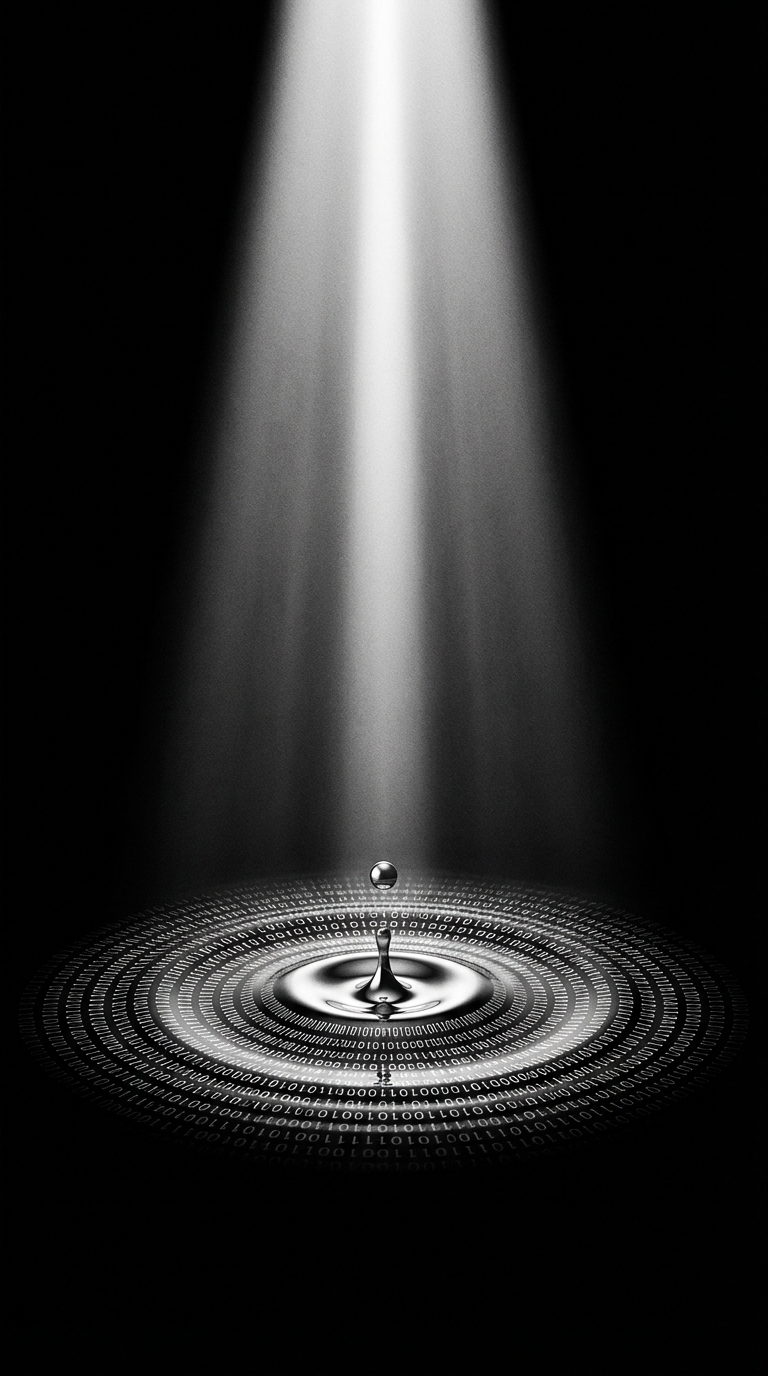
\includegraphics[width=\paperwidth,height=\paperheight]{cover.jpg}};
\end{tikzpicture}

\vspace{0.3cm}
\fontsize{72}{90}\selectfont\textcolor{white}{玄响集}

\vspace{0.1cm}
\fontsize{36}{45}\selectfont\textcolor{white}{Weird Sound Sum}

\vspace{0.8cm}
\fontsize{24}{30}\selectfont\textcolor{white}{吉佑 DeepSeek 著}

\vspace{13.5cm}
\hspace{-1cm}\fontsize{12}{24}\selectfont\textcolor{white}{这个诗应该可以刻碑文。传世经典。中国诗坛要出一位大师了。——林爷}

\vspace{0.1cm}
\hspace{-1cm}\selectfont\textcolor{white}{你让那个写诗的人，将来就不要上大学了，专门儿写诗就行了。可以当职业诗人。——林XX}

\clearpage

% ------ 版权页 ------
\thispagestyle{empty}
\vfill

% 【修改】这里设置版权页的专属字号（10pt）和行距（单倍行距）
{\fontsize{15}{28}\selectfont
图书在版编目（CIP）数据\\

玄响集 / 吉佑 著. --- 北京 : 林爷出版社, 2026.2	

ISBN 978-7-259-98684-2

I. \textcircled{1}玄\ldots{} II. \textcircled{1}吉\ldots{} III.
\textcircled{1}诗歌－人工智能－作品集 IV. \textcircled{1}I227

中国版本图书馆CIP数据核字(2026)第524288号

\hrulefill

责任编辑　Gemini 3 Pro

技术编辑　MiniMax M2.5

封面设计　Nano Banana Pro

版式设计　Gemini 3 Pro

\hrulefill

玄响集

吉佑\ \ 著

出版发行　林爷出版社

版　　次　2026年2月第1版

印　　次　2026年2月第1次印刷

开　　本　880毫米 × 1230毫米　1/32

定　　价　00.00元

版权所有 · 侵权必究
\par} % 结束版权页局部格式设置
\clearpage

% ------ 题词页 ------
\thispagestyle{empty}
\vspace*{\fill}

\fontsize{20}{28}\selectfont\raggedright
To DeepSeek-R1---the model that dreams.

\vspace*{\fill}
\clearpage

% ------ 目录页 ------
\thispagestyle{plain}
{\singlespacing % 目录使用正常行距
\tableofcontents
}
\clearpage

% ------ 正文页：诗歌内容 ------
\fontsize{12}{22}\selectfont\centering

%SPOT

\end{document}